\documentclass[11pt,twoside]{scrartcl}
\usepackage{mdas}
\usepackage{tikz}
\usetikzlibrary{shapes.geometric,tqft}

% We should need this if we stick to v2.0
% \usepackage{tqft}
% \tikzset{
%   tqft/use nodes=false,
% }

\lstset{
numbers=left,
numberstyle=\small,
numbersep=8pt,
frame = single,
language=tex,
framexleftmargin=15pt}

\begin{document}
\title{Drawing TQFT Diagrams}
% If you contribute to the handout, put your name in comment here

\author{Manoj Das}
\org{}
\date{Spring, 2024}
\maketitle
The complete documentation for the \emph{TQFT} package is available at \url{https://mirrors.rit.edu/CTAN/macros/latex/contrib/tqft/tqft.pdf}.
\section{Usage}
To use the \emph{TQFT} package add the following to the preamble of the latex file.
\begin{lstlisting}
    \usepackage{tikz}
    \usetikzlibrary{shapes.geometric,tqft}
\end{lstlisting}
\subsection{Basic Example}
Here is a basic example showing how the \emph{TQFT} package is used within \emph{tikzpicture}, how styles are set, and then the usage of \emph{\textbackslash{}pic} command.

\vspace{1em}
\begin{minipage}[]{0.65\linewidth}
\begin{lstlisting}
    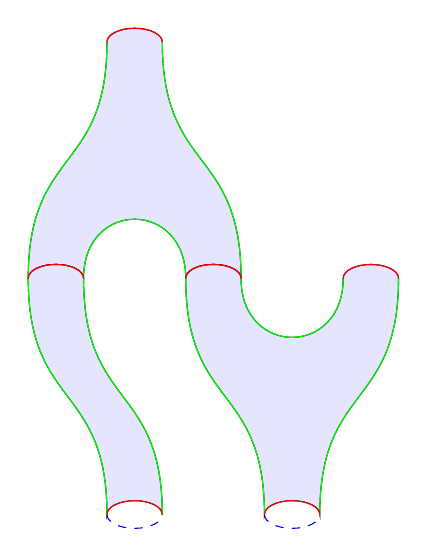
\begin{tikzpicture}[
        tqft,
        cobordism/.style= {
            draw, fill=blue!10
        },
        cobordism edge/.style= {
            draw, green
        },
        every lower boundary component/.style = {
            draw, blue, dashed 
        },
        every upper boundary component/.style = {
            draw, red, solid 
        },
        cobordism height=3cm,
        ]
        \pic [tqft/pair of pants, name=a];
        \pic [tqft/cylinder to next, name = c,
            anchor=incoming boundary 1,
            at=(a-outgoing boundary 1)];
        \pic [tqft/reverse pair of pants, name=c,
            anchor=incoming boundary 1,
            at=(a-outgoing boundary 2)];
    \end{tikzpicture}    
\end{lstlisting}
\end{minipage}
\begin{minipage}[]{0.35\linewidth}
% draw=line color, fill=fill color, 
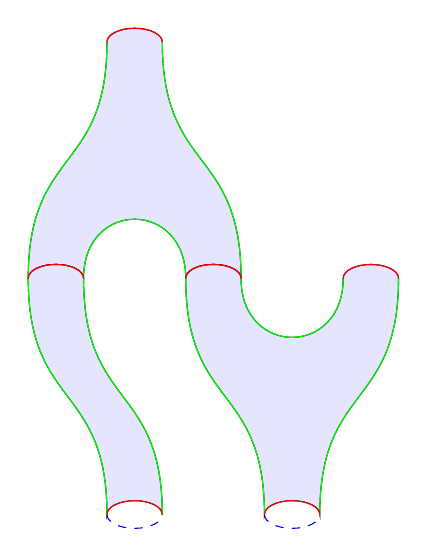
\begin{tikzpicture}[
    tqft,
    cobordism/.style={
        draw,
        fill=blue!10
    },
    cobordism edge/.style={
        draw,
        green
    },
    every lower boundary component/.style =
    {
        draw, 
        blue, 
        dashed 
    },
    every upper boundary component/.style =
    {
        draw, 
        red, 
        solid 
    },
    cobordism height=3cm,
    ]
    \pic [tqft/pair of pants, name=a];
    \pic [tqft/cylinder to next, name = c,
        anchor=incoming boundary 1,
        at=(a-outgoing boundary 1)];
    \pic [tqft/reverse pair of pants, name=c,
        anchor=incoming boundary 1,
        at=(a-outgoing boundary 2)];
\end{tikzpicture}
\end{minipage}
\subsection{Predefined Shapes}
The following predefined shapes are available:
\begin{enumerate}
    \item pair of pants
    \item reverse pair of pants
    \item cylinder to next
    \item cylinder to prior
    \item cylinder
    \item cap
    \item cup
\end{enumerate}
The first 3 are shown in the basic example above.
\subsection{General Shape}
A general shape is a \emph{cobordism}  is a cobordism between a number of incoming circles and a number of outgoing circles, where the numbers of boundary components can be specified as options to the shape. General shape is controlled by following keys (for full list see documentation):
\begin{enumerate}
    \item incoming boundary components
    \item skip incoming boundary components
    \item outgoing boundary components
    \item skip outgoing boundary components
    \item genus - number of holes in the shape
    \item offset - offsets the first outgoing boundary component horizontally relative to the first incoming boundary component
\end{enumerate}
For example,
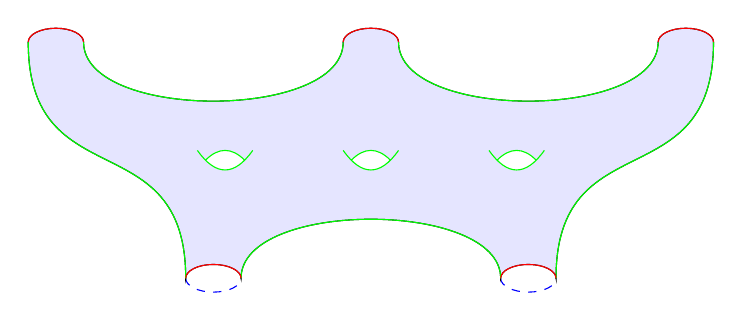
\begin{tikzpicture}[
    tqft,
    cobordism/.style={
        draw,
        fill=blue!10
    },
    cobordism edge/.style={
        draw,
        green
    },
    every lower boundary component/.style =
    {
        draw, 
        blue, 
        dashed 
    },
    every upper boundary component/.style =
    {
        draw, 
        red, 
        solid 
    },
    cobordism height=3cm,
    ]
    \pic [tqft,
            incoming boundary components=5,
            skip incoming boundary components={2,4},
            outgoing boundary components=3,
            skip outgoing boundary components=2,
            offset=1,
            genus=3,
            name=a, 
        ];
\end{tikzpicture}
is produced by
\begin{lstlisting}
    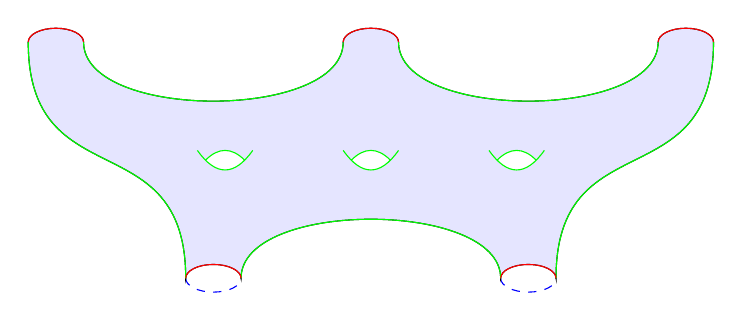
\begin{tikzpicture}[
        tqft,
        cobordism/.style={
            draw,
            fill=blue!10
        },
        cobordism edge/.style={
            draw,
            green
        },
        every lower boundary component/.style =
        {
            draw, 
            blue, 
            dashed 
        },
        every upper boundary component/.style =
        {
            draw, 
            red, 
            solid 
        },
        cobordism height=3cm,
        ]
        \pic [tqft,
                incoming boundary components=5,
                skip incoming boundary components={2,4},
                outgoing boundary components=3,
                skip outgoing boundary components=2,
                offset=1,
                genus=3,
                name=a, 
            ];
    \end{tikzpicture}
\end{lstlisting}

Further, the shapes may be rotated by providing a \emph{rotate} key.
\subsection{Reuse Shape}
We can use \emph{\textbackslash{}tikzset} to define a \emph{pic} and then use the defined picture multiple times.
\begin{remark}
    This is a general \emph{tikz} usage issue. Should see if we can find more examples to get this usage better understood.
\end{remark}
For example, let's define \emph{mtqft} using:

\begin{lstlisting}
\tikzset{
  mtqft/.pic = {
    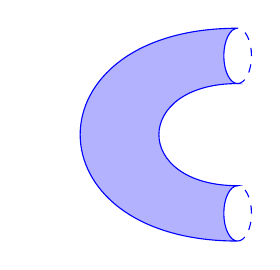
\begin{tikzpicture}[
        tqft,
        cobordism/.style= {
            draw, blue, fill=blue!30
        },
        every lower boundary component/.style = {
                draw, blue, dashed 
            }, 
        cobordism height=4cm,
        ]
        \pic [tqft, 
            incoming boundary components=0,
            outgoing boundary components=2,
            name=a, 
            rotate=90
        ];
    \end{tikzpicture}
    }
}
\end{lstlisting}

\tikzset{
  mtqft/.pic = {
    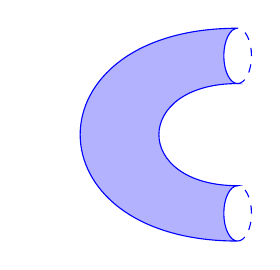
\begin{tikzpicture}[
        tqft,
        cobordism/.style= {
            draw, blue, fill=blue!30
        },
        every lower boundary component/.style = {
                draw, blue, dashed 
            }, 
        cobordism height=4cm,
        ]
        \pic [tqft, 
            incoming boundary components=0,
            outgoing boundary components=2,
            name=a, 
            rotate=90
        ];
    \end{tikzpicture}
    }
}
Then we can use it wherever we need using
\begin{lstlisting}
    \begin{tikzpicture}
        \pic{mtqft};
    \end{tikzpicture}
\end{lstlisting}
For example, this is the first use 
\begin{tikzpicture}
    \pic{mtqft};
\end{tikzpicture}
and here is the second use
\begin{tikzpicture}
    \pic{mtqft};
\end{tikzpicture}
.
\section{Example - 2.3.1}
Recall the definition

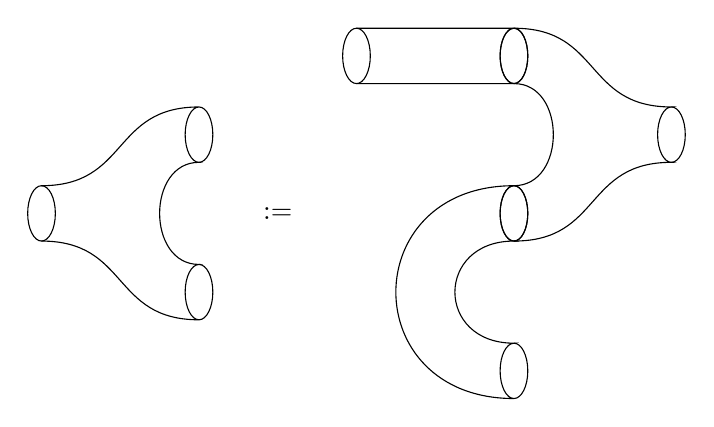
\begin{tikzpicture}[
    tqft,
    cobordism/.style={
        draw,
    },
    every lower boundary component/.style =
    {
        draw,
    },
    % cobordism height=3cm,
    ]
    \pic [tqft/pair of pants, at={(0,-2)}, name=a, rotate=90];
    \node [at={(3,-2)}] {:=};
    \pic [tqft/cylinder, at={(4,0)}, name=b, rotate=90];
    \pic [tqft/reverse pair of pants, name=c, rotate=90,
        anchor=incoming boundary 2,
        at=(b-outgoing boundary 1)];
    \pic [tqft, name=d, rotate=90,
        cobordism height=3cm,
        incoming boundary components=0,
        outgoing boundary components=2,
        anchor=outgoing boundary 2,
        at=(c-incoming boundary 1)];
\end{tikzpicture}
.

The above is produced by
\begin{lstlisting}
    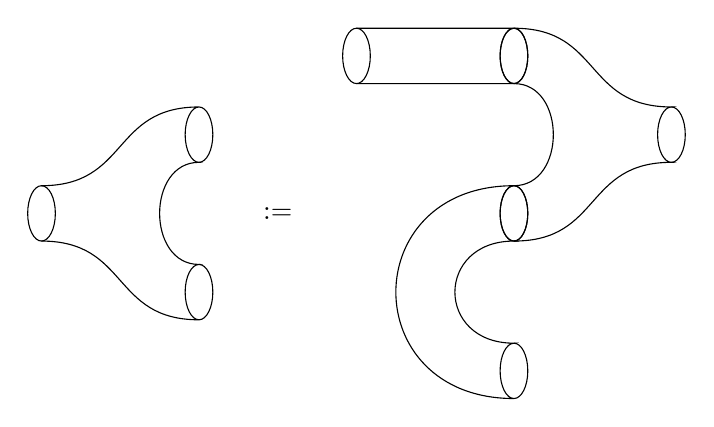
\begin{tikzpicture}[
        tqft,
        cobordism/.style={
            draw,
        },
        every lower boundary component/.style =
        {
            draw,
        },
        ]
        \pic [tqft/pair of pants, at={(0,-2)}, name=a, rotate=90];
        \node [at={(3,-2)}] {:=};
        \pic [tqft/cylinder, at={(4,0)}, name=b, rotate=90];
        \pic [tqft/reverse pair of pants, name=c, rotate=90,
            anchor=incoming boundary 2,
            at=(b-outgoing boundary 1)];
        \pic [tqft, name=d, rotate=90,
            cobordism height=3cm,
            incoming boundary components=0,
            outgoing boundary components=2,
            anchor=outgoing boundary 2,
            at=(c-incoming boundary 1)];
    \end{tikzpicture}    
\end{lstlisting}
\end{document}